\documentclass{beamer}
\usetheme{afm}

\title{Monte Carlo and \\ \vspace{0.25cm}Stochastic Processes}
\author{Matteo Sani - \href{mailto:matteo.sani@unisi.it}{matteo.sani@unisi.it}}

\begin{document}
\begin{frame}[plain]
	\maketitle
\end{frame}

\begin{frame}{Random Variables}
	\begin{itemize}
		\item A random variable is a variable whose values depend on outcomes of a random phenomenon.
        \begin{itemize}
        \item coin toss: only two outcomes are possible: heads or tails;
        \item random variable to represent the result of three dice rolls: it could be somewhere between 3 (1+1+1) and 18 (6+6+6).
        \end{itemize}

        \item Other Examples:
        \begin{itemize}
            \item In the corporate world, random variables can be assigned to: average price of an asset over a given time period, return on investment after a specified number of years, the estimated turnover rate at a company within the following six months. 
            \item Risk analysts assign random variables to risk models when they want to estimate the probability of an adverse event occurring.
        \end{itemize}
	\end{itemize}
\end{frame}

\begin{frame}{Random Variables}
	\begin{itemize}
		\item The \emph{variable} $x$ in an algebraic equation is an unknown value that can be calculated 
        \begin{equation*}
        10 + x = 13 \implies x=3
        \end{equation*}
        \item A \emph{random variable} $X$ has a set of values, and \textbf{any of those values could be the resulting outcome each of them with a certain probability} (probability density function PDF).
	\end{itemize}
\end{frame}

\begin{frame}{Random Variables}
    \begin{columns}
    \column{0.3\textwidth}
    When the range of possible values for $X$ is infinite it is called a \emph{continuous}; contrary it is \emph{discrete}.
    \column{0.7\textwidth}
    \begin{figure}[h]
    \begin{center}
    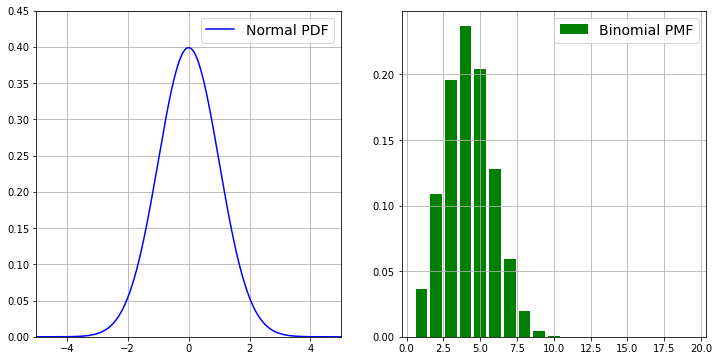
\includegraphics[width=1.0\linewidth]{rv_pdf}
    \end{center}
    \end{figure}    
    \end{columns}
\end{frame}

\begin{frame}{CDF and Quantiles}
	\begin{itemize}
    \item The cumulative distribution function (CDF) $F$ of a random variable $X$ (with PDF $f(x)$, evaluated at $x$, is the probability that $X$ will take a value less than or equal to $x$
    \begin{equation*}
        \begin{gathered}
            F_X(x) = Pr(X\leq x) = \int_{-\infty}^{x} f(x)dx\\
            Pr(a \leq X\leq b) = \int_{-\infty}^{b} f(x)dx - \int_{-\infty}^{a} f(x)dx = \int_{a}^{b} f(x)dx
        \end{gathered}
    \end{equation*}
    
    \item The quantile function $Q$, associated with a probability distribution of a random variable, and evaluated in $\hat{p}$ specifies the value $x$ of the random variable such that the probability of the variable being less than or equal to $x$ equals the given probability $\hat{p}$. 
    \begin{itemize}
        \item It is also called the percent-point function (PPF) or inverse cumulative distribution.
    \end{itemize}
    \begin{equation*}    
        Q_X(p) = F_X^{-1}(X \leq x_{\hat{p}})\;\;\textrm{where}\; F_X(x_{\hat{p}}) = \hat{p}
    \end{equation*}
    
    \item The quantile function does the "inverse" of the cumulative distribution function.
	\end{itemize}
\end{frame}

\begin{frame}{CDF and Quantiles}
    \begin{figure}[h]
    \begin{center}
    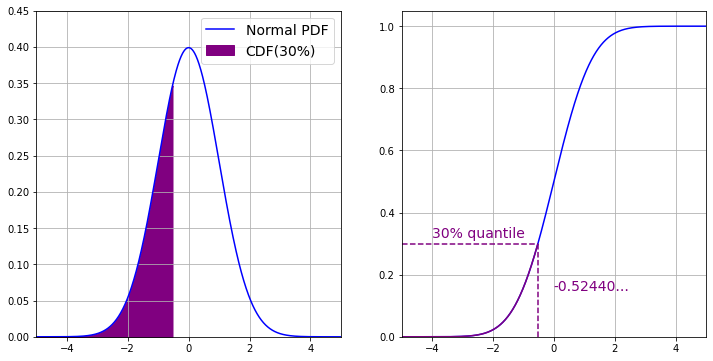
\includegraphics[width=0.7\linewidth]{cdf_quantiles}
    \end{center}
    \end{figure}    
\end{frame}

\begin{frame}[fragile]{PDFs in \texttt{python}}
    Many distributions are implemented in \texttt{scipy} package,
\begin{ipython}
from scipy.stats import norm, binom
     
norm.pdf(0)                 # evaluate the PDF in 0
binom(12, 0.35).pmf(2)      # evaluate the PDF in 0
norm.cdf(0)                 # compute the CDF up to 0
norm.ppf(0.3)               # return the 0.3 quantile
norm.rvs(size=100)          # sample 100 times from normal distribution
\end{ipython}
\end{frame}

\begin{frame}{Monte Carlo Simulation}
    \begin{itemize}
    \item Monte Carlo (MC) methods are a broad class of computational algorithms that rely on repeated random sampling to obtain numerical results
    \begin{itemize}
        \item use randomness to solve problems that might be deterministic in principle;
        \item used when a closed-form solution for a property being studied cannot be developed (i.e. the probability of varying outcomes cannot be determined because of random variable interference). 
     \end{itemize}
    \item In Monte Carlo each random variable of a model is "replaced" with their PDF; the outcome of the model is then computed many times with different samples of the random variables. 
    \item In finance MC has a vast array of potential applications
    \begin{itemize}
        \item to estimate the likelihood that an asset price will move in a certain way;
        \item to assess the risk that an entity will default;
        \item to analyze derivatives such as options.
     \end{itemize}
    \item MC simulations have also countless applications in gaming, meteorology, astronomy, physics...
    \end{itemize}
\end{frame}

\begin{frame}{Algorithm Description}
    \begin{enumerate}
    \item Identify the random variables of the problem and define the domain $\Omega$ of possible inputs (probability distributions for each random variable);
    \item generate random samples from the domain $\Omega$;
    \item compute the model output based on the randomly generated inputs;
    \item repeat the experiment $N$ times and "aggregate" the results.
    \end{enumerate}
    \begin{block}{Example}
    Simulate results of rolling a die. The random variable describe the die outcome, hence $\Omega = {1,2,3,4,5,6}$ with uniform PDF (fair die).
    The simulation consists of sampling uniform distributed integers between 1 and 6.
    \end{block}
\end{frame}

\begin{frame}{Pseudo-Random Numbers}
    \begin{itemize}
    \item  Depending upon the number of uncertainties and their PDFs, a Monte Carlo simulation could involve thousands or even tens of thousands of recalculations.
    \item For each simulation large amounts of random numbers sampled from many different probability distributions are computed, hence the widespread of this method spurred the development of pseudo-random number generators. 
    \item Every programming language has libraries that allows to produce huge series of random numbers:
    \begin{itemize}
        \item those numbers are generated by algorithms that take as input a \emph{seed} which determines univokely the series; 
        \item setting the same seed produce the same set of numbers every time (which is great for debugging purpouses).
    \end{itemize}
    \end{itemize}
\end{frame}

\begin{frame}[fragile]{Pseudo-Random Numbers}  
\begin{ipython}
from numpy import uniform, seed, randint, choice

seed(1)
print(uniform())       # 0.13436424411240122
print(uniform())       # 0.8474337369372327

seed(2)
print(uniform())       # 0.9560342718892494
print(uniform())       # 0.9478274870593494

seed(1)
print(uniform())       # 0.13436424411240122
print(uniform())       # 0.8474337369372327

print (randint(1, 6)) # 1

a = ['a', 'b', 'c', 'd']
print (choice(a, 2, replace=False))  # ['c', 'a']
\end{ipython}
\end{frame}

\begin{frame}[fragile]{Estimate Distributions}
The \texttt{random} module has also some limited capabilities for sampling from a distribution, anyway 
better to use \texttt{scipy}.

\begin{columns}
\column{0.5\linewidth}
\begin{ipython}
from numpy.random import randint
from scipy.stats import norm

# uniform distribution
numbers = []
for _ in range(10000):
    numbers.append(randint(0, 5))

# faster and easier solution
numbers = randint(0, 5, size=10000)    
    
# normal distribution
norm.rsv(size=100000)   
\end{ipython}
\column{0.5\linewidth}    
\begin{figure}[h]
    \begin{center}
    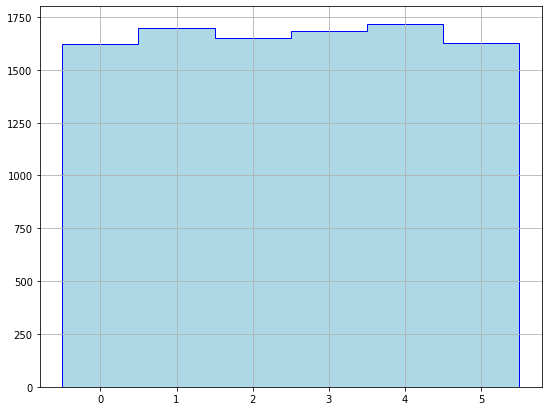
\includegraphics[width=0.55\linewidth]{uniform_distro}\\
    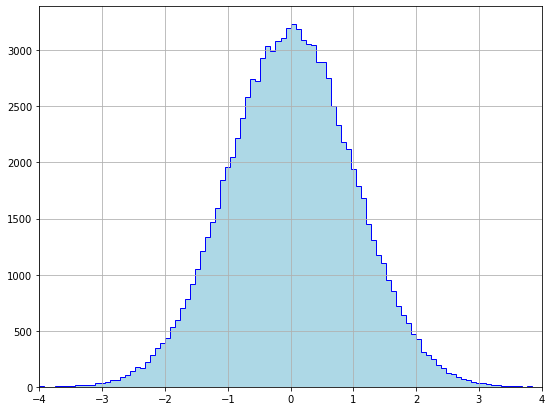
\includegraphics[width=0.55\linewidth]{gauss_distro}
    \end{center}
\end{figure}    
\end{columns}
\end{frame}

\begin{frame}{Monte Carlo Simulation Example}
\begin{block}{Example}
Measure probability to get two kings drawing randomly two cards from a deck.
\begin{equation*}
P_{\textrm{two kings}} = \frac{4}{40} \cdot \frac{3}{39} = \frac{1}{130} \approx 0.007692
\end{equation*}
This analytical results can be reproduced with a Monte Carlo simulation by taking a frequentist approach
\begin{equation*}
\textrm{probability of event} = \cfrac{\textrm{n. successes}}{\textrm{n. experiments}}
\end{equation*}
\end{block}

\end{frame}

\begin{frame}{Monte Carlo Simulation Example}
\begin{itemize}
    \item In the example we ran 10000 simulations and obtained a probability of 0.7\% (it means on average we get 2 kings once every 700 draws).
    \item \emph{The precision of the result depends on the number of "successes".}
    \item Imagine to run only 100 experiments, it is highly probable that I get no successes at all, should I conclude there is a 0 probability to get 2 kings ?
    \item The lower is the probability for a successful experiment the higher has to be the number of simulations, if the probability is small, we need to try many times.
    \item Monte Carlo Simulation is not always the best approach to follow !
\end{itemize}
\href{https://colab.research.google.com/drive/1cQbX7jWk4_pfrm72r3ZiZyDEpevP63z2?authuser=1\#scrollTo=b05dd876\&line=1\&uniqifier=1}{\beamergotobutton{Monte Carlo Simulation}}
\end{frame}

\begin{frame}{Accuracy of Monte Carlo Simulation}
Imagine you don't know the probability of getting two consecutive K from a deck: what can be concluded from the result of a single MC experiment ?
\begin{block}{Central Limit Theorem}    
If $Y_1, Y_2,\dots, Y_n$ are $n$ random samples from a distribution $Y$ with true mean $\mu$ and variance $\sigma^{2}$, then when $n$ is sufficiently large, 
\begin{equation*}
\mu_n = \cfrac{1}{n}\sum_i^n Y_i \approx \mathcal{N}(\mu, \sigma^2/n)
\end{equation*}
has approximately a normal distribution $\mathcal{N}(\mu, \sigma^2/n)$. 

This means that if ones repeats a MC experiment (changing the seed of the random number generator) she should obtain results normally distributed around the \emph{true} value $\mu$.
\end{block}
\href{https://colab.research.google.com/drive/1cQbX7jWk4_pfrm72r3ZiZyDEpevP63z2?authuser=1\#scrollTo=0ef8c284\&line=7\&uniqifier=1}{\beamergotobutton{Monte Carlo Accuracy}}
\end{frame}

\begin{frame}{Central Limit Theorem}
\begin{block}{Consequences}
\begin{enumerate}
	\item The \emph{mean} of our experiment results is the best estimate of $\mu$;
	\item the standard deviation of $\mu_n$ is given by the sample standard deviation ($\sigma_{Y_i}$) divided by the square root of the sample size (\emph{standard deviation of the sample mean}). Hence, the sample mean is much less volatile than the sample values themselves.\textbf{ Consequently, the error reduces at the rate of 1 over the square root of the sample size.} 
\end{enumerate}
\end{block}
\vspace{0.5 cm}
Think for a moment about the implications of point (2).
\end{frame}

\begin{frame}{Monte Carlo Technique Limits}
\begin{itemize}
\item Suppose $\sigma$ is the standard deviation of the experiment results (we did $n_1$ experiments):
\begin{equation*}
\sigma_{\mu_{n_1}} = \cfrac{\sigma}{\sqrt{n_1}}
\end{equation*}
\item Now suppose we wanted to reduce that uncertainty in half. How much larger must the sample be? Let this new sample size be $n_2$. 
\begin{equation*}
	\sigma_{\mu_{n_2}} = \cfrac{\sigma}{\sqrt{n_2}}
\end{equation*}
\item Now note that,
\begin{equation*}
\cfrac{1}{2}\cfrac{\sigma}{\sqrt{n_1}}  = \cfrac{\sigma}{\sqrt{n_2}} \implies n_2 = 4 n_1
\end{equation*}
\item Thus, to achieve a 50\% reduction in error, i.e., a 50\% increase in accuracy, we must \textbf{quadruple} the number of random experiments.
\end{itemize}
\end{frame}

\begin{frame}{Confidence Interval}
\begin{itemize}
\item Since
\begin{equation*}
\mu_n \approx \mathcal{N}(\mu, \sigma^2/n)\implies \mu_n - \mu \approx \mathcal{N}(0, \sigma^2/n)
\end{equation*}
we can define an interval such that there is a given probability to find $\mu$ in there.
\begin{columns}
\column{0.5\linewidth}
\begin{equation*}
P\left(\mu_n - 1.96\frac{\sigma}{\sqrt{n}}\le \mu \le \mu_n + 1.96\frac{\sigma}{\sqrt{n}}\right) = 0.95
\end{equation*}
This is the \emph{95\% confidence interval} since pink area is 95\% of the area under the Gaussian.
\column{0.5\linewidth}
\begin{figure}[h]
    \begin{center}
    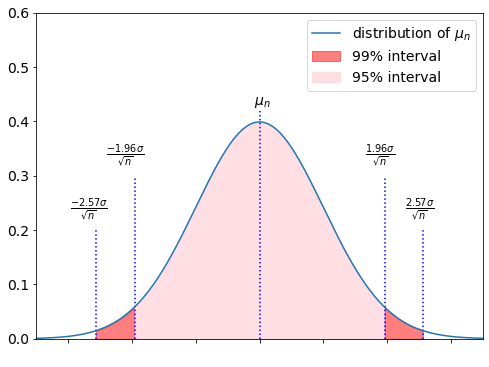
\includegraphics[width=0.8\linewidth]{confidence_interval_pink}
    \end{center}
\end{figure}    
\end{columns}
\item Repeating many times a simulation, the fraction of confidence intervals containing the true $\mu$ would tend toward 95\%.
\end{itemize}
\end{frame}

\begin{frame}[fragile]{Confidence Interval}
  The most common intervals are 99\% and 95\% confidence levels and are respectively defined as $\pm \cfrac{2.57\sigma}{\sqrt{n}}$ and $\pm \cfrac{1.96\sigma}{\sqrt{n}}$.
 \vspace{1.0 cm} 
\begin{ipython}
import numpy as np

cl = 1.96*np.std(r)/np.sqrt(experiments)
print (f"{np.mean(r):.6f} +- {cl:.6f} @ 95% confidence level")
# 0.007689 +- 0.000054 @ 95% confidence level
\end{ipython}
\end{frame}

%\begin{frame}[fragile]{Standard Deviation of the Mean}
%\begin{itemize}
%\item To get further information about the accuracy of the Monte Carlo simulation in general, we can use the standard deviation of the sampled mean. 
%\item Assuming statistical independence of the values in the sample, the standard deviation of the mean is 
%\begin{equation*}
%\sigma _{\text{mean}}={\frac {1}{\sqrt {n}}}\sigma
%\end{equation*}
%where $n$ is the number of observations in the sample used to estimate the mean. 
%
%\begin{ipython}
%print (f"{np.mean(r):.6f} +- {np.std(r)/np.sqrt(experiments):.6f}")
%# 0.007689 +- 0.000028
%\end{ipython}
%\item To get \textbf{one more digit of accuracy (i.e. an error one tenth as large) requires a $\times100$ simulations}.
%\item To get \textbf{three more digits of accuracy requires one million times as much computation}:running 10000 above experiments ($\times10$ more) gives an error 3 times smaller (from 2.8e-5 to about 9e-6).
%\end{itemize}
%\end{frame}

\begin{frame}{Stochastic Processes}
\begin{itemize}
\item \emph{Deterministic process}: all data necessary to predict the system development with 100\% certainty is available.
\item \emph{Stochastic or random process}: exhibits behaviors that cannot be described by a deterministic model, is a \emph{noisy} process where uncertainty needs to be modeled
   \begin{itemize}
    \item it is a collection of random variables indexed by some set (usually time);
    \item each random variable of the stochastic process is uniquely associated with an element in the set. 
    \end{itemize}
\begin{figure}[h]
    \begin{center}
    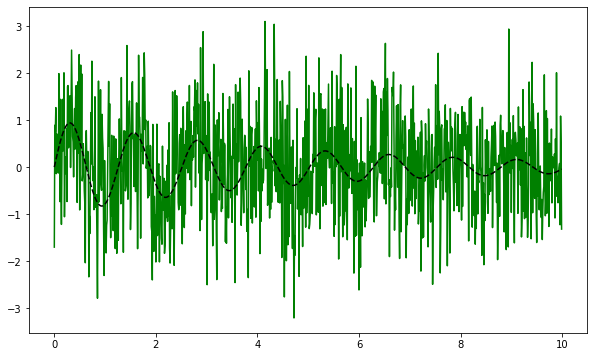
\includegraphics[width=0.5\linewidth]{stochastic_process}
    \end{center}
\end{figure}        
\end{itemize}
\end{frame}

\begin{frame}{Stochastic Processes}
\begin{itemize}
\item Stochastic processes are described by \emph{stochastic differential equation (SDE)}:
\begin{equation*}
dX(t) = \mu(t,X(t)) dt + \sigma(t,X(t)) dW(t) = \underbrace{\mu(t,X(t))dt}_{\textrm{deterministic}} + \underbrace{\sigma(t,X(t)) \mathcal{N}(0,1)\sqrt{dt}}_{\textrm{stochastic}}
\end{equation*}
\item The mean of $dW$ is zero and its variance is $dt$
   \begin{itemize}
    \item the standard deviation grows with the square root of time: $W(t) - \mathcal{N}( 0, t )$ because each $dW$ is distributed like independent standard Gaussian.
    \end{itemize}
\end{itemize}
\begin{figure}[h]
    \begin{center}
    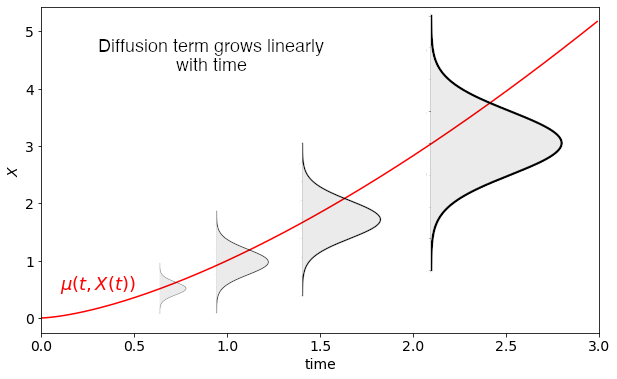
\includegraphics[width=0.50\linewidth]{brownian_process}
    \end{center}
\end{figure}        
\end{frame}

\begin{frame}{Geometric Brownian Motion}
\begin{itemize}
\item Stock prices changes as a result of the random fluctuations given by the trades. The relative change in its price in a period $dt$ can be decomposed into two parts:
\begin{itemize}
    \item \emph{deterministic}, the expected return from the stock hold during the time period $dt$ ($\mu S_tdt$);
    \item \emph{stochastic} which reflects the random changes of the market (e.g. as a response to external effects such as unexpected news). A reasonable assumption is to take this contribution proportional to the stock ($\sigma S_t dW_t$).
\end{itemize}
\begin{equation*}
dS_t = \mu S_tdt + \sigma S_tdW_t;\quad\frac{dS_t}{S_t} = d\textrm{log}(S_t) = \mu dt + \sigma dW_t 
\end{equation*}
\item The solution of this SDE can be derived by applying the It$\hat{o}$'s formula (full derivation in the notes).
\begin{equation*}
S_t = S_{t-1}e^{\big(\mu - \frac{1}{2}\sigma^2\big)dt + \sigma \mathcal{N}(0,1)\sqrt{dt}}
\end{equation*}
\end{itemize}
\end{frame}

\begin{frame}{Geometric Brownian Motion}
\begin{equation*}
	\textrm{log}\left(\cfrac{S_t}{S_{t-1}}\right) = \left(\mu - \frac{1}{2}\sigma^2\right)dt + \sigma \mathcal{N}(0,1)\sqrt{dt} \approx\mathcal{N}\left[\left(\mu-\frac{\sigma^2}{2}\right)T, \sigma^2 T\right]
\end{equation*}
\begin{itemize}
\item  The change in $\textrm{log} S_t$ has a constant \emph{drift} $\mu - \frac{1}{2}\sigma^2$ and a constant variance rate $\sigma^2$ therefore $\textrm{log} S_t$ at some time $T$ is normally distributed with:
\item A variable whose logarithm is normally distributed is said to be \emph{log-normal}.
\end{itemize}
\end{frame}

\begin{frame}{Lognormal Distribution}
\begin{block}{Lognormality}
  \emph{Lognormality} is important because ensures a stock price will never be negative.
  \begin{columns}
    \column{0.5\linewidth}
Looking at the initial $dS$ equation we had that:
\begin{equation*}
dS_t = \mu S_tdt + \sigma S_tdW_t
\end{equation*}
\column{0.4\linewidth}
\begin{figure}[h]
    \begin{center}
    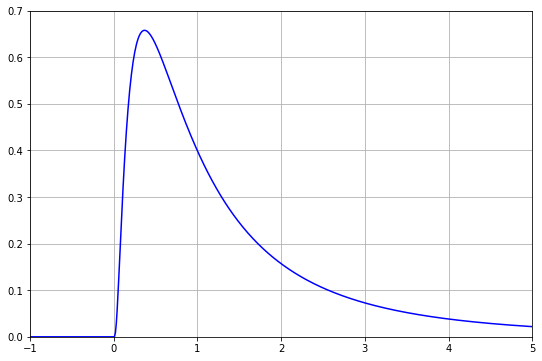
\includegraphics[width=0.85\linewidth]{lognormal}
    \end{center}
\end{figure}        
\end{columns}
which shows that the closer is $S_t$ to 0 the smaller is the $dS$ variation (so it will never go below 0).
\end{block}
\end{frame}

\begin{frame}{Simulating SDE (Euler Scheme)}
\begin{itemize}
\item  Consider the generic SDE
\begin{equation*}
dX(t) = \mu(t,X(t))dt + \sigma(t,X(t))dW(t)
\end{equation*}
the simulation of $X(t)$ is done as follows.
\item Starting from the value of $X(t_i)$ compute $X(t_{i+1})$ using the given SDE by setting $\Delta t = t_{i+1} - t_{i}$, and sampling from a standard normal $\mathcal{N}(0,1)$
\begin{equation*}
X(t_{i+1}) = X(t_i) + \mu(t_i,X(t_i))\Delta t + \sigma(t_i,X(t_i))\sqrt{\Delta t}\mathcal{N}(0,1)
\end{equation*}
\end{itemize}
\end{frame}

\begin{frame}[fragile]{Wiener Process Example}
Let's simulate two possible realization of a Wiener process ($\mu = 0, \sigma=1$)
\begin{equation*}
X(t_{i+1}) = X(t_i) + \sqrt{\Delta t}\mathcal{N}(0,1)
\end{equation*}
\begin{columns}
\column{0.5\linewidth}
\begin{ipython}
from numpy import sqrt, cumsum
from numpy.random import seed, normal

def wiener(dt, steps):
    return normal(size=steps)*sqrt(dt)

seed(10)
w1 = cumsum(wiener(1/365, 1000))
w2 = cumsum(wiener(1/365, 1000))
		\end{ipython}
		\column{0.5\linewidth}
		\begin{figure}[h]
			\begin{center}
				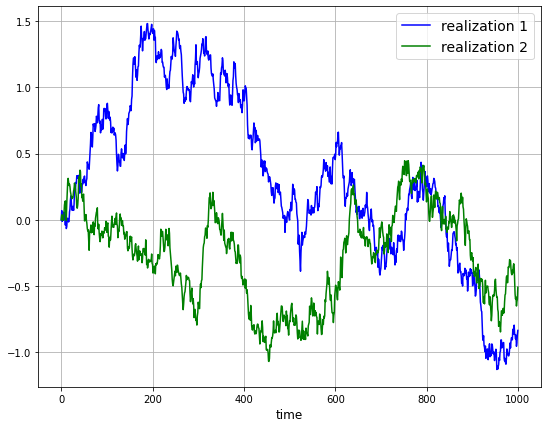
\includegraphics[width=0.90\linewidth]{wiener}
			\end{center}
		\end{figure}
	\end{columns}
\end{frame}

\begin{frame}{Remark on Stochastic Processes}
\begin{itemize}
\item Whenever we want to estimate a quantity involving stochastic processes we have to compute an expectation $\mathbb{E}[f(X)]$.
\item This means that we have to average the value of $f(X)$ among all the possible realizations of $X$ taking into account the probability associated to each path.
\item Monte Carlo simulation is a way of estimate an expectation: 
\begin{enumerate}
\item simulate as many $X$ realization as possible;
\item for each simulation compute $f(X)$;
\item average the results to estimate $\mathbb{E}[f(X)]$.
\end{enumerate}
\end{itemize}
\href{https://colab.research.google.com/drive/1cQbX7jWk4_pfrm72r3ZiZyDEpevP63z2?authuser=1\#scrollTo=1895fa54}{\beamergotobutton{SDE Simulation}}
\end{frame}

\end{document}
